\ifx\FORMAT\undefined
\documentclass[11pt]{book}
\usepackage{amsmath,mathtools}
\usepackage[utf8]{inputenc}
\usepackage[ngerman]{babel}
\usepackage{acronym}
\usepackage{graphicx} 
\usepackage{epstopdf}
\usepackage{svg}
\usepackage{multirow}
\usepackage{amssymb}
\usepackage{trfsigns}
\usepackage{setspace}
\usepackage{yfonts}
%\usepackage{HsKatitle11}

\onehalfspacing


%Hyperlinks package, links aus inhaltsverzeichnis
\usepackage{hyperref}
\hypersetup{
    colorlinks=false, %set true if you want colored links
    linktoc=all,
    linkbordercolor = {white}
}
%Blattformatierung
\usepackage{geometry}
\geometry{a4paper, top=25mm, left=30mm, right=25mm, bottom=20mm}

%Listing
\usepackage{courier}
\usepackage{listings}
\usepackage{color}
 \lstset{
   frame=tb,
   framexleftmargin=2.5em,
   basicstyle=\small\linespread{0.9}\bfseries\ttfamily,
   emph={square}, 
   emphstyle=\color{blue}\texttt,
   emph={[2]root,base},
   emphstyle={[2]\color{yac}\texttt},
   showstringspaces=false,
   flexiblecolumns=false,
   tabsize=2,
   numbers=left,
   numberstyle=\small\bfseries\ttfamily,
   numberblanklines=false,
   stepnumber=1,
   numbersep=10pt,
   xleftmargin=25pt
 }
 
 \def\presuper#1#2%
	{\mathop{}%
	\mathopen{\vphantom{#2}}^{#1}%
	\kern-\scriptspace%
	#2}
%Display vecotr in a reference frame
\newcommand{\vecBS}[4]{\presuper{#1}{\begin{pmatrix}
#2 \\ #3 \\ #4
\end{pmatrix}}}
%Boldsymbol shortcut
\newcommand{\bs}[1]{\boldsymbol{#1}}
%Bezugssystemdefinition
\newcommand{\defBS}[1]{\{#1\} [ \bs{e}_{{#1}_1},\bs{e}_{{#1}_2}, \bs{e}_{{#1}_3} ]}
%Projektionsmatrix
\newcommand{\pMat}[2]{\presuper{#1}{\bs{P}}^{#2}}
%Differenation in Respekt zu BS
\newcommand{\diffIn}[3]{\frac{\presuper{#1}{d{#2}}}{d#3}}
\newcommand{\partialDiffIn}[3]{\frac{\presuper{#1}{\partial{#2}}}{\partial #3}}
%Geschwindigkeit/Beschleunigung
\newcommand{\vel}[3]{\presuper{#1}{\bs{#2}}^{#3}}

%Rightarrow with spaceing
\newcommand{\rArrow}{\hspace{5pt}\rightarrow\hspace{5pt}}
%Inneres Produkt
\newcommand{\inProd}[2]{\langle {#1}, {#2} \rangle}

%System macro
\newcommand{\cSS}[3]{\textfrak{S}($\bs{#1}$,$\bs{#2}$,$\bs{#3}$)}
\newcommand{\dSS}[3]{\textfrak{D}($\bs{#1}$,$\bs{#2}$,$\bs{#3}$)}

%Laplace transform sign with spaces
\newcommand{\myLaplace}{\hspace{15pt}\laplace\hspace{15pt}}

\newcommand*{\signed}[1]{%
        \nolinebreak[3]\hspace*{\fill}\mbox{\emph{#1}}
    }
\begin{document}
\fi

\chapter{Modellbildung für den Würfel auf  einer Kante}\label{chapter_TM_Edge}
Dieses Kapitel widmet sich der Herleitung der Bewegungsgleichungen für den Fall, dass der Würfel auf einer seiner Kanten steht. Hierfür wird Kanes Methodik \cite{KaneBook} angewandt, welche sich in die Untersuchung der kinematischen und kinetischen Gegebenheiten unterteilt. In der Kinematikanalyse werden zunächst generalisierte Koordinaten eingeführt, um die Konfiguration des Systems zu beschreiben. Des Weiteren werden Bezugssysteme verwendet, um einzelne Körper des Gesamtsystems in dem mathematischen Modell darzustellen. Die kinematische Untersuchung endet mit der Definition der generalisierten Geschwindigkeiten und der Bestimmung der partiellen Geschwindigkeiten, welche als Betrag und Richtung der Systembewegung interpretiert werden können.
In dem zweiten Teil des Kapitels wird die Kinetik betrachtet. Zu Beginn werden die resultierenden Drehmomente formuliert, welche auf die verschiedenen Körper wirken. Diese werden verwendet um mit Hilfe der partiellen Geschwindigkeiten die generalisierten aktiven Kräfte $F_i$ zu ermitteln. Analog werden die Trägheitsmomente und daraus die generalisierten Trägheitskräfte $F^*_i$ berechnet, welche mittels Kanes Gleichung $F_i+F^*_i=0$ zu den gesuchten Bewegungsgleichungen führen. Zuletzt wird die Auswirkung der generalisierten Geschwindigkeiten auf die resultierenden Bewegungsgleichungen anhand eines einfachen Beispiels erörtert.
\newpage
\section{Untersuchung der Kinematik}
Der erste Schritt besteht darin die kinematischen Zusammenhänge des Systems zu analysieren. Im Fall, dass der Würfel auf einer Kante balanciert, verfügt dieser über zwei rotatorische Freiheitsgrade. Der erste wird von der generalisierten Koordinate $\varphi$ beschrieben und gibt die Orientierung des Würfelgehäuses wieder. Die zweite generalisierte Koordinate $\psi$ erfasst die Rotation der Schwungmasse relativ zu dem Würfelgehäuse.
\begin{figure}[!ht]
\centering
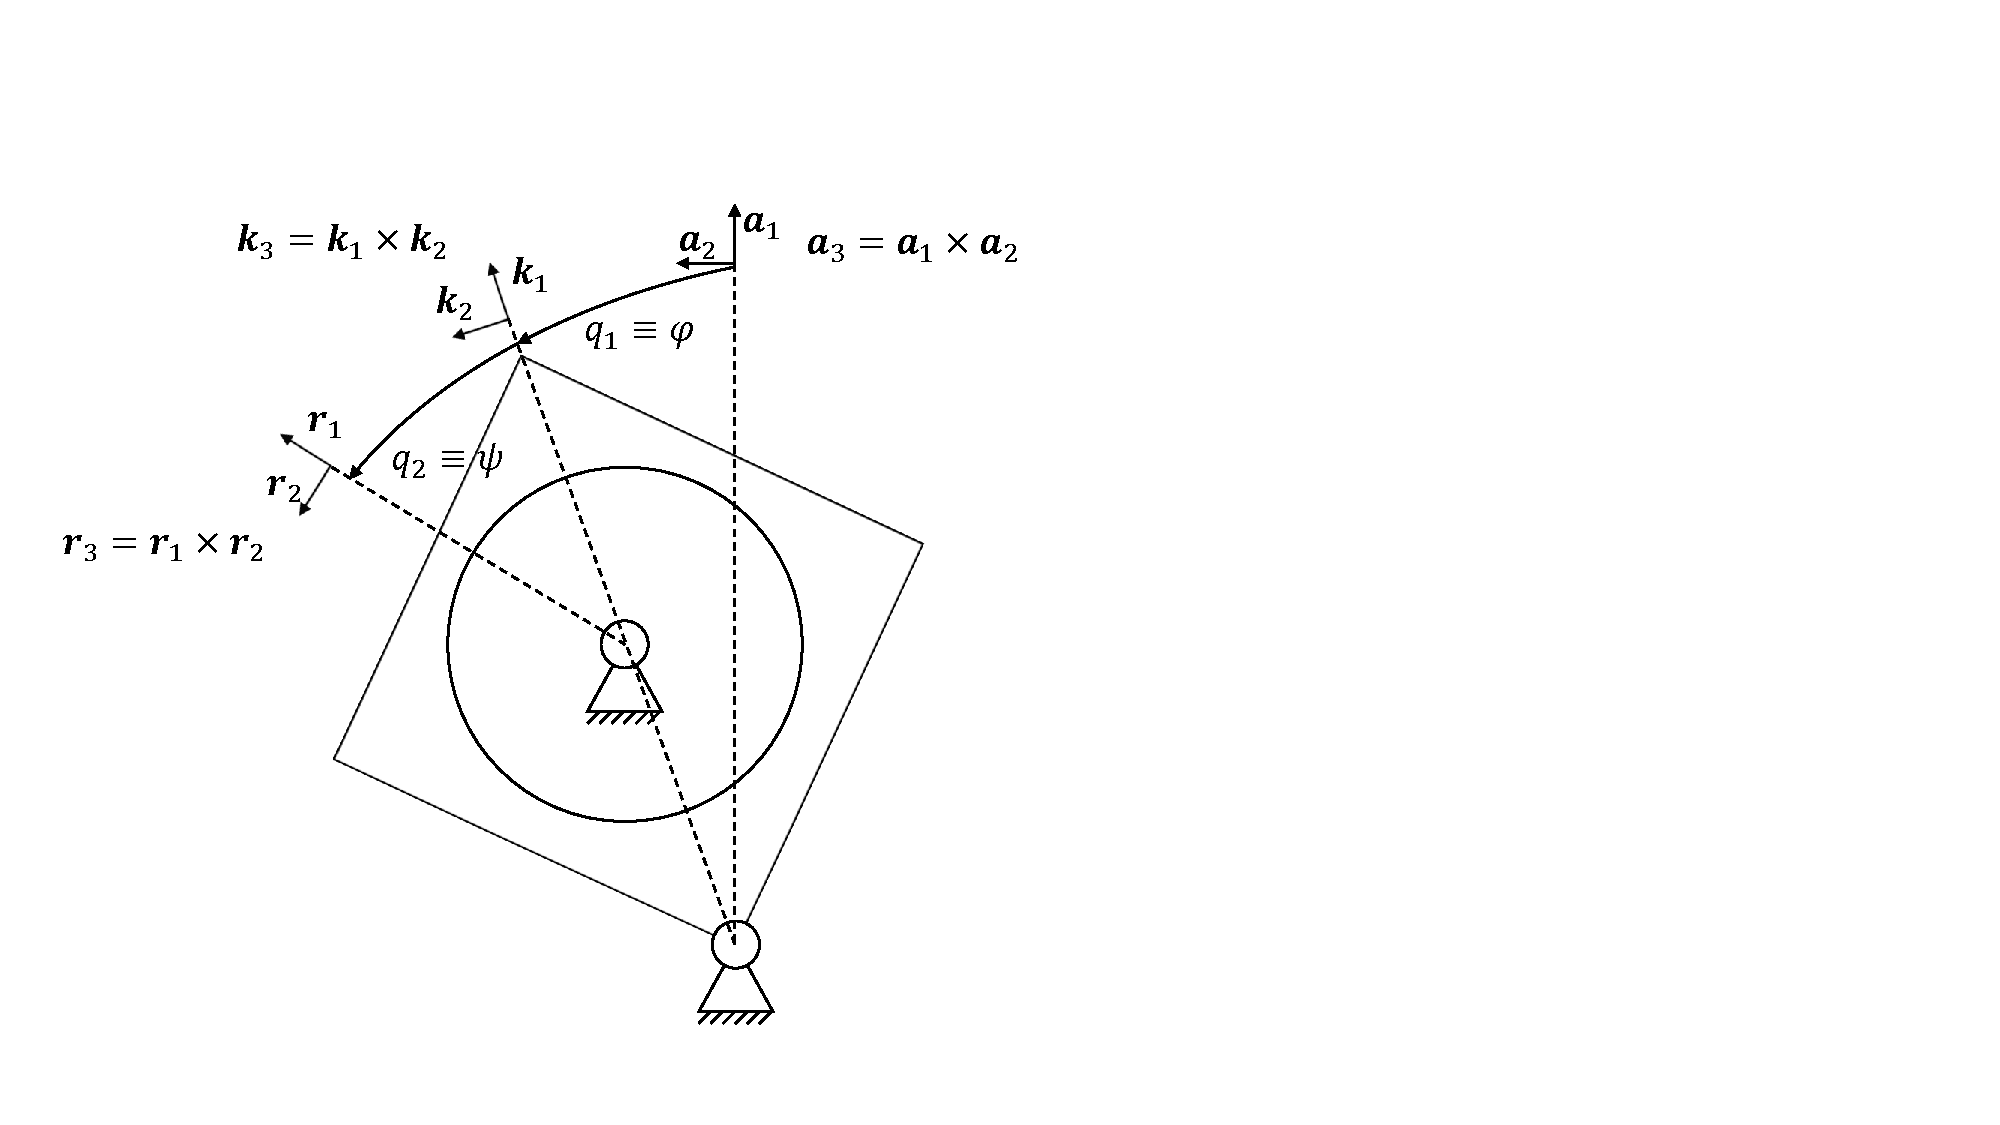
\includegraphics[width=0.6\linewidth, trim={1cm 1.5cm 18cm 3.5cm}, clip]{img/ModellWuerfelseite}
\caption{Kinematikplan des Würfels auf einer Kante, Quelle: eigene Darstellung}
\label{skizze_dynamik_edge}
\end{figure}

Um die Körper des Systems zu modellieren werden im nächsten Schritt die Bezugssysteme $A$, $K$ und $R$ eingeführt, wobei ein beliebiges Bezugssystem $B$ durch drei Vektoren $\bs{b_i} \ i \in \{1,2,3\}$ definiert wird. Die Vektoren $\bs{b_i}$ werden als Vektorbasis bezeichnet.\footnote{Allgemein genügen drei linear unabhängige Vektoren als Vektorbasis, allerdings werden in dieser Arbeit ausschließlich paarweise orthogonale Einheitsvektoren verwendet, da diese eine einfachere Handhabung ermöglichen. Im weiteren Verlauf wird nicht explizit erwähnt, dass es sich bei den Vektorbasen um paarweise orthogonale Einheitsvektoren handelt.} In diesem Fall ist $A$ ein Intertialsystem, das heißt die Ausrichtung der Vektoren $\bs{a_i}$ ist konstant. Deshalb wird $A$ bzw. dessen Vektorbasis auch als raumfest bezeichnet. Bei $K$ handelt es sich um ein körperfestes Bezugssystem, die Vektoren $\bs{k_i}$ sind an dem Würfelgehäuse fixiert und ändern ihre Ausrichtung in Abhängigkeit von $\varphi$. Das Bezugssystem $R$ ist ebenfalls körperfest, wobei die Vektorbasis an der Schwungmasse fixiert ist. Foglich beschreiben die Koordiaten $\varphi$ und $\psi$ die Rotation von $K$ relativ zu $A$ bzw. von $R$ gegenüber $K$. 

Mittels eines Bezugssystems kann ein bliebiger Vektor als Linearkombination der Vektorbasis dargestellt werden. Als Beispiel sei der Ortsvektor $\bs{c}$ des Würfelschwerpunktes geannt, wobei das verwendete Bezugssystem durch den vorangehenden Superskript gekennzeichnet wird.
\begin{equation}
\bs{c} = l\idx{C} \cdot \bs{k}\idx{1} + 0 \cdot \bs{k}\idx{2} + 0 \cdot \bs{k}\idx{3} = \vecBS{K}{l\idx{C}}{0}{0}
\end{equation}
Um nun die Komponenten $\alpha_i$ des Vektors $\bs{c}$ in dem Bezugssystem $A$ zu erhalten, muss das Skalarprodukt $\inProd{\bs{a}_i}{\bs{c}}$ berechnet werden. Wird dieser Ansatz auf alle drei Komponenten appliziert ergibt sich der Zusammenhang\footnote{Um die allgemeine Gültigkeit der linearen Abbildung zu verdeutlichen wird in dieser Gleichung die Definition $\bs{c}=\vecBS{K}{l_C}{0}{0}\equiv\vecBS{K}{\beta_1}{\beta_2}{\beta_3}$ verwendet.}
\begin{equation}
\begin{split}
\bs{c} &= \vecBS{A}{\alpha\idx{1}}{\alpha\idx{2}}{\alpha\idx{3}} = \inProd{\bs{c}}{\bs{a}\idx{1}}\cdot \bs{a}\idx{1} + \inProd{\bs{c}}{\bs{a}\idx{2}}\cdot\bs{a}\idx{2} + \inProd{\bs{c}}{\bs{a}\idx{3}}\cdot\bs{a}\idx{3} 
= \vecBS{A}{\inProd{\bs{c}}{\bs{a}\idx{1}}}{\inProd{\bs{c}}{\bs{a}\idx{2}}}{\inProd{\bs{c}}{\bs{a}\idx{3}}}
\\
&= \vecBS{A}
{\beta\idx{1}\cdot\inProd{\bs{a}\idx{1}}{\bs{k}\idx{1}} + \beta\idx{2}\cdot\inProd{\bs{a}\idx{1}}{\bs{k}\idx{2}} + \beta\idx{3}\cdot\inProd{\bs{a}\idx{1}}{\bs{k}\idx{3}}}
{\beta\idx{1}\cdot\inProd{\bs{a}\idx{2}}{\bs{k}\idx{1}} + \beta\idx{2}\cdot\inProd{\bs{a}\idx{2}}{\bs{k}\idx{2}} + \beta\idx{3}\cdot\inProd{\bs{a}\idx{2}}{\bs{k}\idx{3}}}
{\beta\idx{1}\cdot\inProd{\bs{a}\idx{3}}{\bs{k}\idx{1}} + \beta\idx{2}\cdot\inProd{\bs{a}\idx{3}}{\bs{k}\idx{2}} + \beta\idx{3}\cdot\inProd{\bs{a}\idx{3}}{\bs{k}\idx{3}}}
\\
&= \presuper{K}{\begin{pmatrix}
\underbrace{
\begin{bmatrix}
\inProd{\bs{a}\idx{1}}{\bs{k}\idx{1}} & \inProd{\bs{a}\idx{1}}{\bs{k}\idx{2}} & \inProd{\bs{a}\idx{1}}{\bs{k}\idx{3}} \\
\inProd{\bs{a}\idx{2}}{\bs{k}\idx{1}} & \inProd{\bs{a}\idx{2}}{\bs{k}\idx{2}} & \inProd{\bs{a}\idx{2}}{\bs{k}\idx{3}} \\
\inProd{\bs{a}\idx{3}}{\bs{k}\idx{1}} & \inProd{\bs{a}\idx{3}}{\bs{k}\idx{2}} & \inProd{\bs{a}\idx{3}}{\bs{k}\idx{3}}
\end{bmatrix}}_{\equiv \pMat{K}{A}} \cdot \underbrace{\begin{bmatrix}
\beta\idx{1} \\ \beta\idx{2} \\ \beta\idx{3}
\end{bmatrix}}_{= \presuper{K}{\bs{c}}}
\end{pmatrix}} 
= \presuper{A}{\begin{pmatrix}
\begin{bmatrix}c_{\varphi} & -s_{\varphi} & 0 \\ s_{\varphi} & c_{\varphi} & 0 \\ 0 & 0 & 1 \end{bmatrix} \cdot \presuper{K}{\bs{c}} \end{pmatrix}}\,.
\end{split}
\end{equation}
Somit handelt es sich bei der Projektion eines Vektors, welcher in einem beliebigen Bezugssystem $A$ dargestellt ist, in ein weiteres Bezugssystem $B$ um eine lineare Abbildung. Die Abbildungsvorschrift wird durch die Matrix $\pMat{B}{B}$ definiert. Des weiteren zeigt dieses Beispiel die perspektivische Bedeutung eines Bezugssystem. Wird der Vektor $\bs{c}$ in $K$ dargestellt hängt er lediglich von der Länge $l_C$ ab und ist folglich konstant. Aus der Perspektive von $A$ ist der Vektor eine Funktion von $\varphi$ und somit variabel. Die Begründung hierfür ist, dass das Intertialsystem $A$ die Bewegung des Würfels im Raum wahrnimmt, wodurch der Ortsvektor des Schwerpunktes variable erscheint.
Im Gegensatz dazu erfasst das köperfeste Bezugssystem $K$ einen Vektor aus der Perspektive des Würfelkörpers. Aus diesem Grund ist der in $K$ dargstellte Ortsvektor $\presuper{K}{\bs{c}}$ des Schwerpunktes konstant.
Dieser Umstand kann genutzt werden, indem ein Vektor zunächst in einer einfachen Form dargestellt und anschließend in das gewünschte Bezugssystem projiziert wird. Als Beispiel dient die Berechnung des Gravitationsmoments $\bs{T}^{K/O}$. Der Erdbeschleunigungsvektor $\bs{g}$ ist im Inertialsystem $A$ konstant und wird von dort in das körperfeste System $K$ transformiert.
\begin{equation}
\begin{split}
\bs{T}^{K/O} = \bs{c}\times m\cdot\bs{g} &= \vecBS{K}{l\idx{C}}{0}{0}\times \vecBS{A}{-m\cdot g}{0}{0} = \vecBS{K}{l\idx{C}}{0}{0}\times\presuper{K}{\begin{pmatrix}
\pMat{A}{K}\cdot \vecBS{A}{-m\cdot g}{0}{0}
\end{pmatrix}}
\\
&= \vecBS{K}{l\idx{C}}{0}{0}\times \vecBS{K}{-c_{\varphi}\cdot m\cdot g}{s_{\varphi}\cdot m\cdot g}{0} = \vecBS{K}{0}{0}{s_{\varphi}\cdot m\cdot g\cdot l\idx{C}}
\end{split}
\end{equation}
Dieses Beispiel zeigt, dass die Einführung von Bezugssystemen eine eindeutige Notation und Vorgehensweise zur Berechnung von vektorwertigen Funktionen mit sich bringt. Man möge bei diesem Anwendungsfall argumentieren, dass die trigonometrischen Zusammenhänge des Gravitationsmomentes auch aus der Abbildung \ref{skizze_dynamik_edge} ablesen lassen. Allerdings ist die hier betrachtete Vorgehensweise allgemeingültig und kann auf beliebig komplexe Systeme angewendet werden. Beispielsweise kann das Gravitationsmoment in dem Fall, dass der Würfel auf einer Ecke steht, kaum mehr aus einer Skizze bestimmt werden.

Zur vollständigen Beschreibung der Kinematik müssen die Geschwindigkeiten des Systems ermittelt werden, welche aus den Ableitungen der Winkel $\varphi$ und $\psi$ hervorgehen. Als Beispiel für die Ableitung eines Vektors dient wieder der Ortsvektor $\bs{c}$ des Schwerpunktes. Dieser ist aus der Perspektive des Bezugssystem $K$ konstant, folglich verschwindet auch dessen Ableitung bzw. Geschwindigkeit. Wird der Vektor aber in $A$ abgebildet hängt dieser von der Zeitfunktion $\varphi(t)$ ab. Deshalb muss bei der Ableitung eines Vektors das Bezugssystem angegeben werden, aus dessen Perspektive differenziert wird ([Kane], S.25ff). Wenn $\bs{c}$ in $A$ differenziert werden soll, so muss dieser zunächst in $A$ dargestellt und anschließend komponentenweise nach der Zeit abgeleitet werden.
\begin{equation}
\frac{\presuper{A}{d}\bs{c}}{dt} = \frac{d(c_{\varphi}\cdot l\idx{C})}{dt}\cdot \bs{a}\idx{1} + \frac{d(s_{\varphi}\cdot l\idx{C})}{dt}\cdot \bs{a}\idx{2} + \frac{d(0)}{dt}\cdot \bs{a}\idx{3} = \vecBS{A}{-s_{\varphi}\cdot \dot{\varphi}\cdot l\idx{C}}{c_{\varphi}\cdot \dot{\varphi}\cdot l\idx{C}}{0}
\end{equation}
Hieraus folgt, dass auch die Geschwindigkeiten eines Körpers lediglich als relativ zu einem Bezugssystem angegeben werden können. Somit beschreibt $\vel{B}{v}{P}$ die Geschwindigkeit bzw. $\vel{B}{a}{P}$ die Beschleunigung  eines Punktes oder Körpers $P$  relativ zu einem Bezugssystem $B$. Diese werden wie folgt definiert ([Kane], S.28).
\begin{equation}
\vel{B}{v}{P} = \frac{\presuper{B}{d\bs{p}}}{dt} \hspace{35pt} \vel{B}{a}{P} = \frac{\presuper{B}{d}\vel{B}{v}{P}}{dt}
\end{equation}
Die selbe Notation wird für Winkelgeschwindigkeiten und -beschleunigungen eingeführt, wobei $\vel{A}{\omega}{B}$ die Winkelgeschwindigkeit und $\vel{A}{\alpha}{B}$ die Winkelbeschleunigung eines Punktes oder Bezugssystems $B$ relativ zu $A$ ist. Die Geschwindigkeit relativ zu einem Inertialsystem wird auch als absolute Geschwindigkeit bezeichnet. Für die Bezugssysteme $K$ und $R$ lassen sich mit Hilfe der Abbildung \ref{skizze_dynamik_edge} die folgenden Winkelgeschwindigkeiten bestimmen, wobei die absolute Winkelgeschwindigkeit eines Bezugssystems die Summe seiner relativen Winkelgeschwindigkeiten ist ([Kane], S.24f).
\begin{equation}
\vel{A}{\omega}{K} = \vecBS{K}{0}{0}{\dot{\varphi}} \hspace{15pt} \vel{K}{\omega}{R} = \vecBS{R}{0}{0}{\dot{\psi}} \hspace{15pt} \vel{A}{\omega}{R} = \vel{A}{\omega}{K} + \vel{K}{\omega}{R} = \vecBS{A}{0}{0}{\dot{\varphi} + \dot{\psi}}
\end{equation}
Der letzte Schritt bei der Untersuchung der Kinematik besteht darin die  generalisierten Geschwindigkeiten zu definieren und daraus die partiellen Geschwindigkeiten zu berechnen. Bei den generalisierten Geschwindigkeiten $u_i$ handelt es sich um skalare Größen deren Anzahl gleich der Zahl der generalisierten Koordinaten ist. Die generalsierten Geschwindigkeiten sind für gewöhnlich abhängig von den Zeitableitungen der generalisierten Geschwindigkeiten $\dot{q}_i$, wobei sie so gewählt werden müssen, dass die Definitionen eindeutig nach den Ableitungen $\dot{q}_i$ aufgelöst werden können. Die Einführung der generalisierten Geschwindigkeiten verfolgt das Ziel, möglichst einfache Ausdrücke für die absoluten Geschwindigkeiten $\vel{A}{\omega}{K}$ und $\vel{A}{\omega}{R}$ und, wie sich im späteren Verlauf zeigen wird, einfachere Ausdrücke der Bewegungsgleichungen zu erhalten. Deshalb werden hier die  Definitionen 
\begin{equation}
\begin{split}
u\idx{1} = u\idx{K} \equiv \dot{\varphi} &\hspace{35pt} u\idx{2} = u\idx{R} \equiv \dot{\varphi} + \dot{\psi} \\
\vel{A}{\omega}{K} = \vecBS{K}{0}{0}{u\idx{1}} & \hspace{35pt} \vel{A}{\omega}{R}=\vecBS{K}{0}{0}{u\idx{2}}
\end{split}
\end{equation}
gewählt. Diese Geschwindigkeitsausdrücke können auch in die Form
\begin{equation}
\vel{A}{\omega}{K} = u\idx{1}\cdot \vel{A}{\omega}{K}\idx{1} + u\idx{2} \cdot \vel{A}{\omega}{K}\idx{2} \hspace{35pt} \vert \hspace{15pt} \vel{A}{\omega}{K}\idx{1} = \bs{k}\idx{3}, \hspace{10pt} \vel{A}{\omega}{K}\idx{2} = \bs{0}
\end{equation}
\begin{equation}
\vel{A}{\omega}{R} = u\idx{1}\cdot \vel{A}{\omega}{R}\idx{1} + u\idx{2} \cdot \vel{A}{\omega}{R}\idx{2} \hspace{35pt} \vert \hspace{15pt} \vel{A}{\omega}{R}\idx{1} = \bs{0}, \hspace{10pt} \vel{A}{\omega}{R}\idx{2} = \bs{k}\idx{3}
\end{equation}
gebracht werden, wobei die Größen $\vel{A}{\omega}{K}_i$ und $\vel{A}{\omega}{R}_i$ partielle Geschwindigkeiten genannt werden. Diese Zerlegung kann so interpretiert werden, dass die generalisierten Geschwindigkeiten $u_i$ als skalare Größen den Betrag der Bewegung und die entsprechende partielle Geschwindigkeit, als vektorielle Größe, deren Richtung wiedergibt. Die Vorteile diese Zerlegung in generalisierte und partielle Geschwindigkeiten wird sich im folgenden Abschnitt zeigen.

\newpage
\section{Untersuchung der Kinetik}
Im nächsten Schritt wird die Kinematik des Systems untersucht, um die Bewegungsgleichungen herzuleiten. Hierfür werden zunächst die Drehmomente analysiert, welche auf den Würfelgehäuse und die Schwungmasse wirken. Letztere wird einerseits von dem Motormoment $\bs{T}^{R/M}_M$ beschleunigt, andererseits wirkt ein verzögerndes Reibmoment $\bs{T}^{R/M}_M$. Das Reibmoment wird als proportional zu der Winkelgeschwindigkeit $\dot{\psi}$ modelliert.
\begin{equation}
\bs{T}^{R/M} = \bs{T}^{R/M}_M + \bs{T}^{R/M}_R = [T_M - C_{\psi}(u_2 - u_1)]\cdot \bs{k}_3
\end{equation}
Das Motor- und Reibmoment wirken an dem Verbindungspunkt zwischen Schwungmasse und Würfelgehäuse. Deshalb beeinflussen die beiden den Würfelkörper in umgekehrter Richtung. Des weiteren wird das Würfelgehäuse von dem Gravitationsmoment $\bs{T}^{K/O}_G$ beschleunigt. Die Summe der Komponenten ergibt das resultierende Drehmoment $\bs{T}^{K/O}$.
\begin{equation}
\bs{T}^{K/O} = T^{K/O}_G - \bs{T}^{R/M}_M - \bs{t}^{R/M}_R = [m\cdot g\cdot l_C\cdot s_{\varphi} - T_M + C_{\psi}(u_2 - u_1)] \cdot \bs{k}_3
\end{equation}
Um die Bewegungsgleichungen zu ermitteln, werden die generalisierten aktiven Kräfte $F_i$ benötigt. Hierfür werden die Skalarprodukte der Drehmomente, welche auf die Körper wirken, und die partiellen Winkelgeschwindigkeiten, des entsprechenden Körpers, berechnet. Die Summe über alle Körper ergibt die generalisierte aktive Kraft $F_i$.
\begin{equation}
\begin{split}
F_1 &= \inProd{\bs{T}^{K/O}}{\vel{A}{\omega}{K}_1} + \inProd{\bs{T}^{R/M}}{\vel{A}{\omega}{R}_1}
 = m\cdot g\cdot l_C\cdot s_{\varphi} - T_M + C_{\psi}(u_2 - u_1)
\\
F_2 &= \inProd{\bs{T}^{K/O}}{\vel{A}{\omega}{K}_2} + \inProd{\bs{T}^{R/M}}{\vel{A}{\omega}{R}_2} = T_M - C_{\psi}(u_2 - u_1)
\end{split}
\end{equation}
Die partiellen Geschwindigkeiten können als Bewegungsrichtungen der Körper interpretiert werden. Somit stellen die generalisierten Kräfte $F_i$ den Beitrag der Drehmomente in die jeweilige Bewegungsrichtung wieder.

Als Gegenstück zu den generalisierten aktiven Kräften müssen nun die generalisierten Trägheitskräfte $F^*_i$ ermittelt werden. Das resultierende Trägheitsmoment der Schwungmasse ergibt sich aus dem Produkt des Skalars $I_R$, welcher das Massenträgheitsmoment des Körpers relativ zu $M$ beschreibt, und der Winkelbeschleunigung $\vel{A}{\alpha}{R}$.\footnote{Die hier verwendete Berechnung ist nicht allgemeingültig. Für gewöhnlich wird zur Berechnung der Trägheitsmomente ein Trägheitstensor $\bs{I}$ verwendet. Die in einem späteren Kapitel erläutert.}
\begin{equation}
\bs{T}^{R/M}_* = -I_R\cdot \vecBS{K}{0}{0}{\dot{u}_2}
\end{equation}
Das Trägheitsmoment des Würfelkörpers berechnet sich aus dessen Trägheitsskalar $I_K$ und der Winkelbeschleunigung $\vel{A}{\alpha}{K}$. Die Größe $I_K$ ist die Summe des Massenträgheitsmoments des Würfelgehäuses $I^{GH/O}$ und dem Einfluss der Schwungmasse, wleche dabei als Punkt mit der Masse $m_R$ und dem Abstand $l_{MO}$ betrachtet wird.
\begin{equation}
\bs{T}^{K/O}_* = -(I^{GH/O} + m_R\cdot l^2_{MO})\cdot \vecBS{K}{0}{0}{\dot{u}_1} = -I_K\cdot \vecBS{K}{0}{0}{\dot{u}_1}
\end{equation}
Die generalisierten Trägheitskräfte $F^*_i$ werden wieder aus der folgenden Summe von Skalarprodukten berechnet.
\begin{equation}
\begin{split}
F^*_1 &= \inProd{\bs{T}^{K/O}_*}{\vel{A}{\omega}{K}_1} + \inProd{\bs{T}^{R/M}_*}{\vel{A}{\omega}{R}_1} = -I_K\cdot \dot{u}_1 
\\
F^*_2 &= \inProd{\bs{T}^{K/O}_*}{\vel{A}{\omega}{K}_2} + \inProd{\bs{T}^{R/M}_*}{\vel{A}{\omega}{R}_2} = -I_R\cdot \dot{u}_2 
\end{split}
\end{equation}
Die Bewegunsgleichungen resultieren nun aus Kanes Gleichung $F_i + F^*_i = 0$.
\begin{equation}
\begin{split}
F_1 + F^*_1 = 0 &\hspace{15pt}\leftrightarrow\hspace{15pt} I_K\cdot \dot{u}_1 = m\cdot g\cdot l_C\cdot s_{\varphi} - T_M + C_{\psi}(u_2 - u_2) 
\\
F_2 + F^*_2 = 0 &\hspace{15pt}\leftrightarrow\hspace{15pt} I_R\cdot \dot{u}_2 = T_M - C_{\psi}(u_2 - u_1)
\end{split}
\end{equation}


Rückblickend kann Kanes Methodik in die folgenden Schritte unterteilt werden. Zunächst wird die Kinematik des Systems analysiert, wobei die Körper mit Hilfe von Bezugssystemen modelliert werden. Die Definition von generalisierten Geschwindigkeiten ermöglicht die Bestimmung der partiellen Geschwindigkeiten, wodurch die Bewegung des Systems in eine Art Betrag und Richtung unterteilt wird. Anschließend werden die partiellen Geschwindigkeiten genutzt um die wirkenden Kräfte und Trägheitskräfte in die Bewegungsrichtungen zu projizieren. Hieraus resultieren die generalisierten aktiven Kräfte und generalisierten Trägheitskräfte, welche mittels Kanes Gleichung auf die gesuchten Bewegungsgleichungen führen.

Um die Bedeutung der generalisierten Geschwindigkeiten zu verdeutlichen wird der Fall betrachtet, dass die folgende Definition gewählt wird.
\begin{equation}
\tilde{u}_1 \equiv \dot{\varphi} \hspace{35pt} \tilde{u}_2 \equiv \dot{\psi}
\end{equation}
\begin{equation}
\begin{split}
\vel{A}{\tilde{\omega}}{K}_1 = \bs{k}_3 &\hspace{35pt} \vel{A}{\tilde{\omega}}{K}_2 = 0
\\
\vel{A}{\tilde{\omega}}{R}_1 = 0 &\hspace{35pt} \vel{A}{\tilde{\omega}}{R}_2 = \bs{k}_3
\end{split}
\end{equation}
\begin{equation}
\begin{split}
\tilde{F}_1 = m\cdot g\cdot l_C\cdot s_{\varphi} &\hspace{35pt} \tilde{F}_2 = T_M - C_{\psi}(u_2-u_1) 
\\
\tilde{F}^*_1 = -I_R\cdot (\dot{\tilde{u}}_1 + \dot{\tilde{u}}_2) - I_K\cdot \dot{\tilde{u}}_1 &\hspace{35pt} \tilde{F}^*_2 = -I_R\cdot (\dot{\tilde{u}}_1 + \dot{\tilde{u}}_2)
\end{split}
\end{equation}
\begin{equation}
\begin{split}
\tilde{F}_1 + \tilde{F}^*_1 = 0 &\hspace{15pt}\leftrightarrow\hspace{15pt} I_k\cdot \dot{\tilde{u}}_1 + I_R\cdot (\dot{\tilde{u}}_1+\dot{\tilde{u}}_2) = m\cdot g\cdot l_C\cdot s_{\varphi} 
\\
\tilde{F}_2 + \tilde{F}^*_2 = 0 &\hspace{15pt}\leftrightarrow\hspace{15pt} I_R\cdot (\dot{\tilde{u}}_1+\dot{\tilde{u}}_2) = T_M - C_{\psi}(\dot{\tilde{u}}_2 - \dot{\tilde{u}}_1)
\end{split}
\end{equation}
Dieses Beispiel zeigt, dass die Wahl der generalisierten Geschwindigkeiten eine direkte Auswirkung auf die Form der resultierenden Bewegungsgleichungen hat. Zwar kann die letztere mittels $u_1 = \tilde{u}_1 \ ,\ u_2 = \tilde{u}_1 + \tilde{u}_2$ und dem Einsetzen der zweiten in die erste Gleichung in die ursprüngliche Form überführt werden. Allerdings stellt die Modellierung des Würfels auf einer Ecke einen Anwendungsfall dar, bei dem der Berechnungsaufwand durch eine geschickte Wahl der generalisierten Geschwindigkeiten drastisch reduziert werden kann.

\ifx\FORMAT\undefined
\end{document}
\fi